%!TEX root = paper.tex

%NYC.gov \cite{nycgov} reports statistics and datasets for a range of domains such as emergency incidents, non-emergency events, crimes, offenses and more. To ensure public safety and smooth functioning of the city, it is important to allocate resources for these types of events efficiently. Particularly, response times for emergency incidents can be reduced and improve the logistics of the office in charge. NYC Open Data portal and the Office of Emergency Management (OEM) provide the Emergency Response Incidents dataset, which is publicly available at \cite{nycopendata} and is updated daily.

A number of emergency incidents (e.g. fire, building collapse, etc.) are reported on a regular basis in cities around the world. It is important that city officials are able to allocate sufficient resources to ensure public safety, smooth functioning of cities and address such incidents in a timely manner.  To  engage the public in coordinating these emergency response services smoothly, governments and city officials have made such data openly available to everyone. By adopting a data-driven approach, cities can efficiently allocate resources,  plan prudently, and thus minimize the loss to human life and property and improve resolution time. 

One of the major challenges in this regard is estimating the resolution time for  emergency events in the future. While emergencies are unpredictable by nature and often happen unexpectedly, it is possible to leverage past resolution time data to predict the resolution time of future events. This is because the nature of the event (e.g., fire), the extent of damage, and the number of personnel and equipment available on site are keys factors that dictate the total time needed to address the issue. For example, if multiple emergencies occur in a colocated manner, then it is likely that the time needed to address each of these issues will be higher than usual because of the division of resources. Therefore, if a data-driven analysis suggests that resolution time for future events will be higher than a desired value for a particular incident type, then this analysis can provide insights into budget spending, personnel hiring, and resource allocation.


Hence, in this paper, we design \textbf{DeepER}, a deep learning based emergency resolution time prediction system that predicts the future resolution time of incidents based on historical data. We consider three important emergency incident types, namely, \textit{Fire}, \textit{Law} and \textit{Structural}. We model emergency resolution time prediction as a time series prediction problem. At the core of DeepER there is a sequence-to-sequence encoder-decoder neural network architecture. Both the encoder and the decoder in DeepER are Recurrent Neural Networks (RNNs) and the basic cell is an LSTM cell. The encoder receives the previous resolution times as input and encodes them into a hidden context vector. This hidden vector is given as an input to the decoder, which generates future resolution times.

To evaluate the performance of DeepER, we perform extensive experiments on the publicly available NYC Emergency Response Incidents dataset \cite{nycopendata}. We use the data for a period of approximately eight years for the three incident types. This dataset is challenging from the perspective of time series analysis and prediction because emergency events by nature occur at random times (i.e., lack periodicity), have limited correlation to each other and may not follow seasonal trends. Because of this reason, we design DeepER as a sequence-to-sequence model so that it can unearth  the dependencies among the data points in the sequence even though the time period between two consecutive events in the sequence is varying. DeepER leverages these hidden patterns in data to make superior predictions.

%, where each incident type has multiple sub types. 
%Different sets of fixed number of consecutive events do not occur in a fixed-time period. %In other words, the number of events for each incident type differ within days, months and years. 
%The incidents for which response times are recorded do not occur in a fixed time interval. This non-equidistant characteristic of the dataset makes the prediction task challenging, specially in the search of dynamic-length patterns. 

We compare the performance of DeepER with two widely used baselines--- Linear Regression and Auto Regressive Integrated Moving Average (ARIMA). We use two metrics to evaluate the models--- Root Mean Squared Error (RMSE) and Mean Absolute Error (MAE). DeepER achieves an average performance improvement of 3\% and 16\% with respect to RMSE and 10\% and 27\% with respect to MAE  over ARIMA and Linear Regression, respectively. Our results demonstrate that DeepER is a practically viable system that provides superior prediction performance and can be used to aid city planning and management. We conclude the paper with a discussion of some of the insights we obtain while conducting this investigation.

The rest of the paper is organized as follows. In Section \ref{sec:related}, we present related work. We present  the dataset and discuss the problem investigated in this paper in Section \ref{sec:data}. We then describe the DeepER system in Section \ref{sec:model} and the implementation details in Section \ref{sec:implementation}. We present experimental results in Section \ref{sec:results} and discuss some of our insights from this work in Section \ref{Data:Discussion}.

%Our main contributions are as follows:
%
%\begin{itemize}
%\item We propose \textit{DeepER}, a deep learning based emergency response prediction system, that uses past data to predict future response times. \textit{DeepER} is an encoder-decoder based system which consists of two components --- an encoder which is a Long Short Term Me
%\end{itemize}


\begin{figure*}[!ht]
    \centering
  \subfloat[Fire]{%
       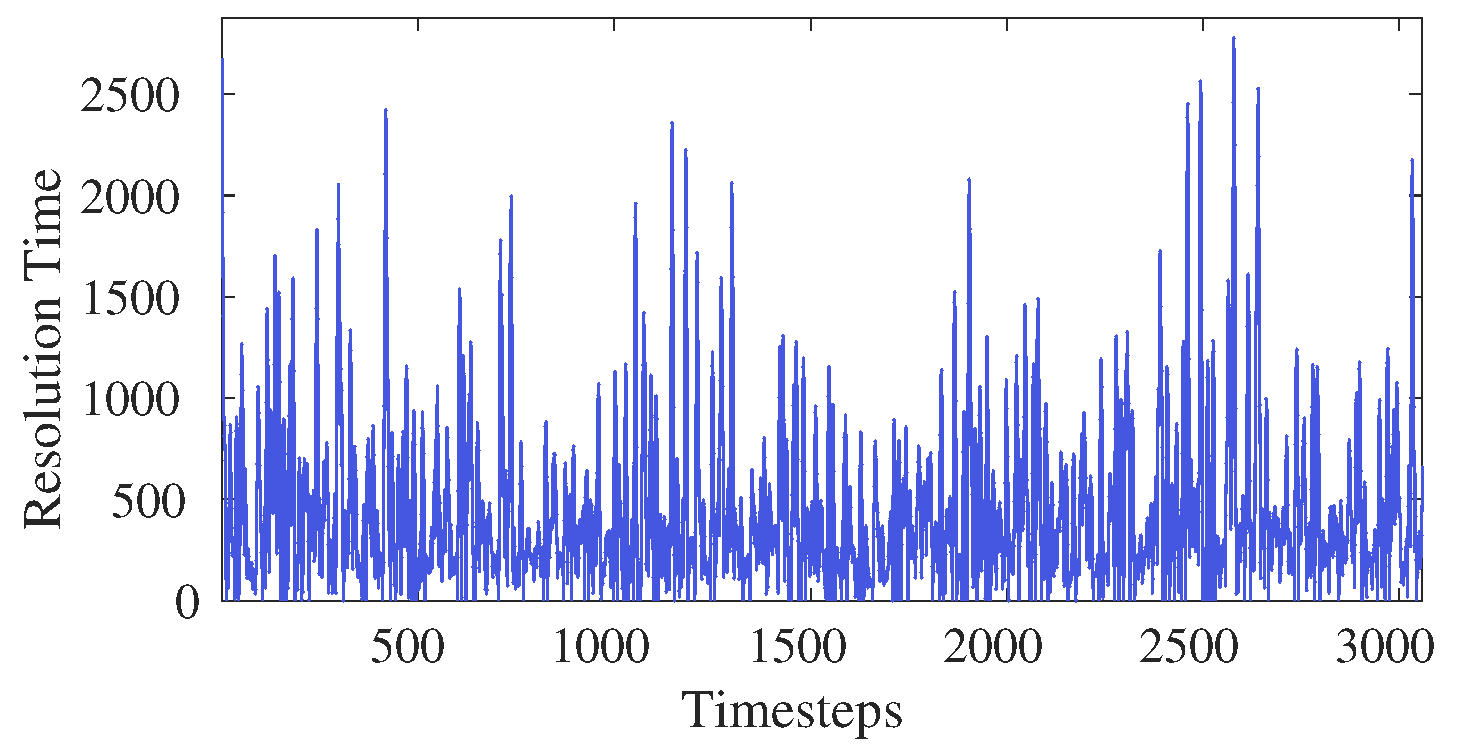
\includegraphics[scale=0.23]{Figures/Data/FullData/Fir}
       \label{1a}}
  \subfloat[Law]{%
       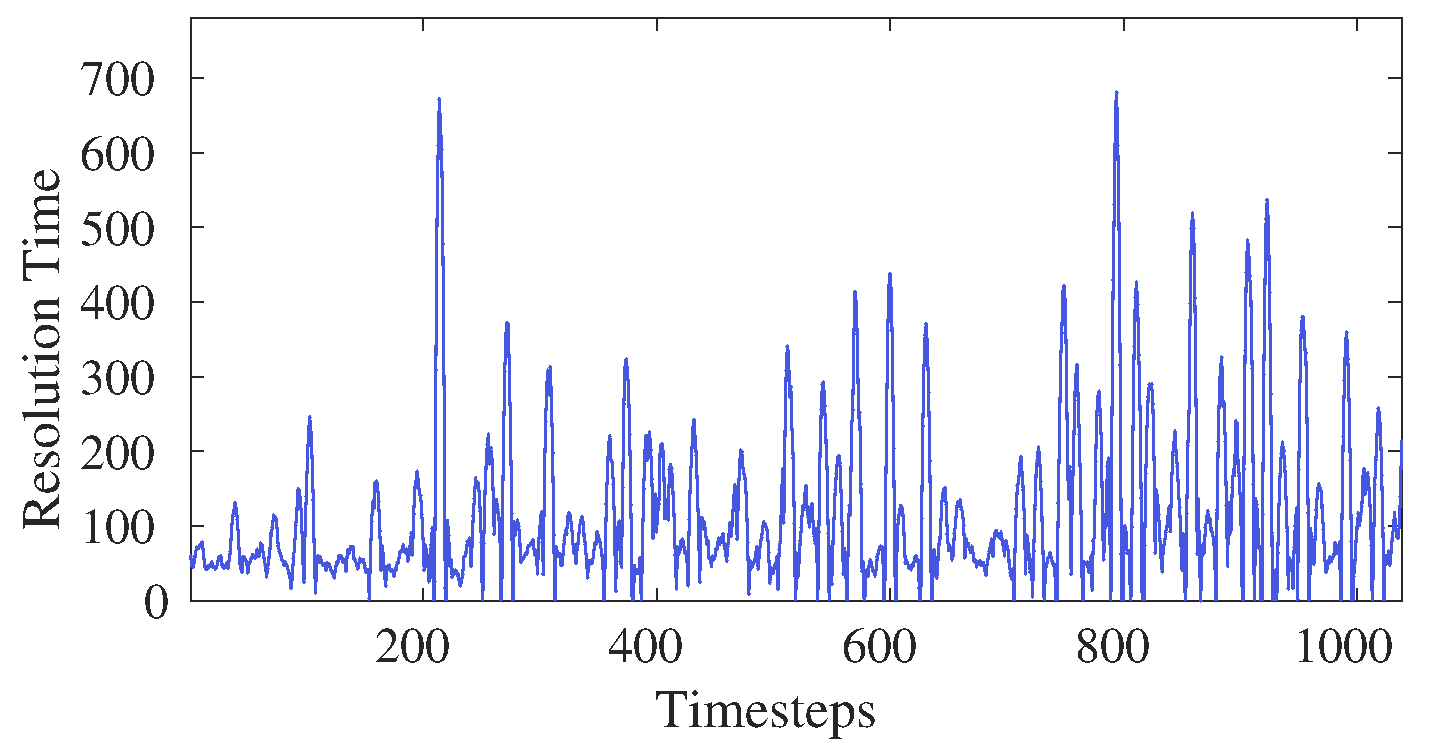
\includegraphics[scale=0.23]{Figures/Data/FullData/Law}
       \label{1b}}
  \subfloat[Structural]{%
       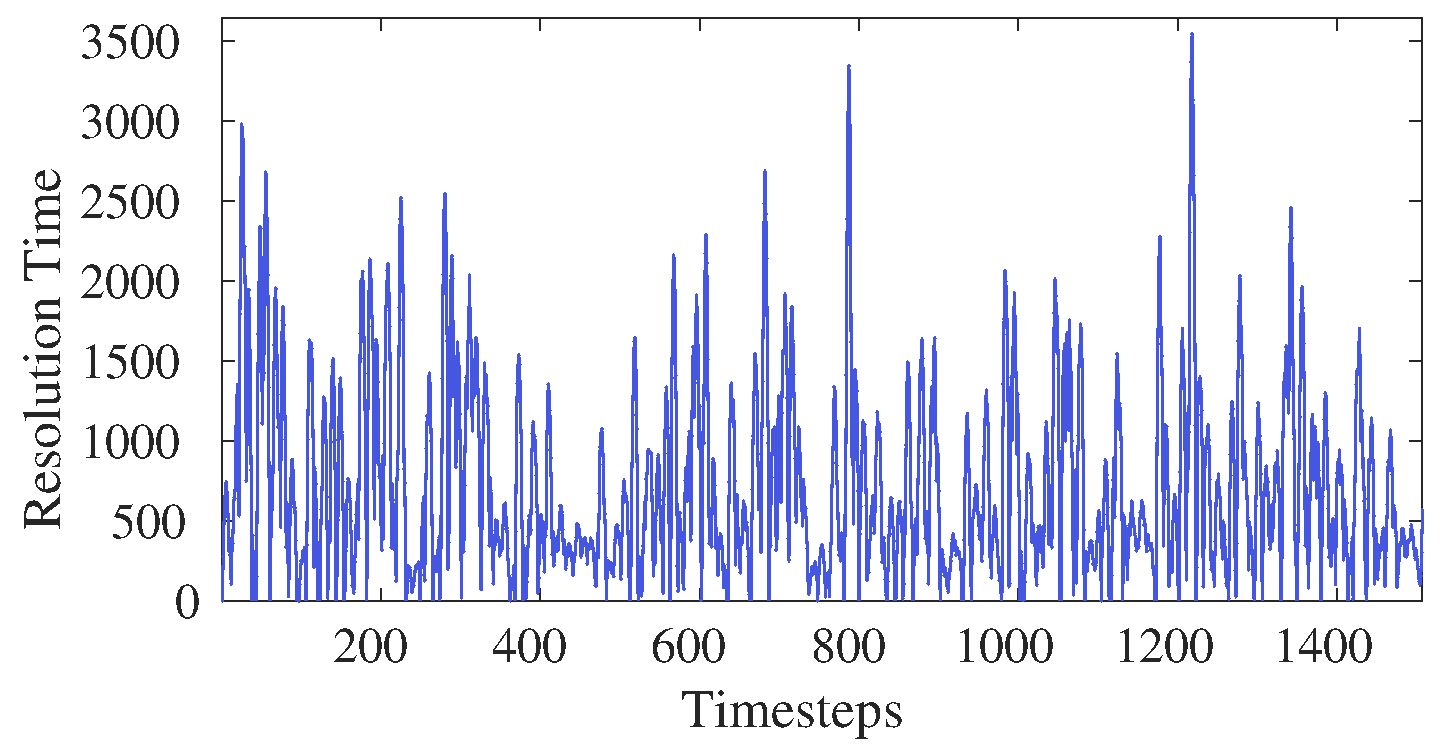
\includegraphics[scale=0.23]{Figures/Data/FullData/Str}
       \label{1c}}
  %\subfloat[Utility]{%
  %     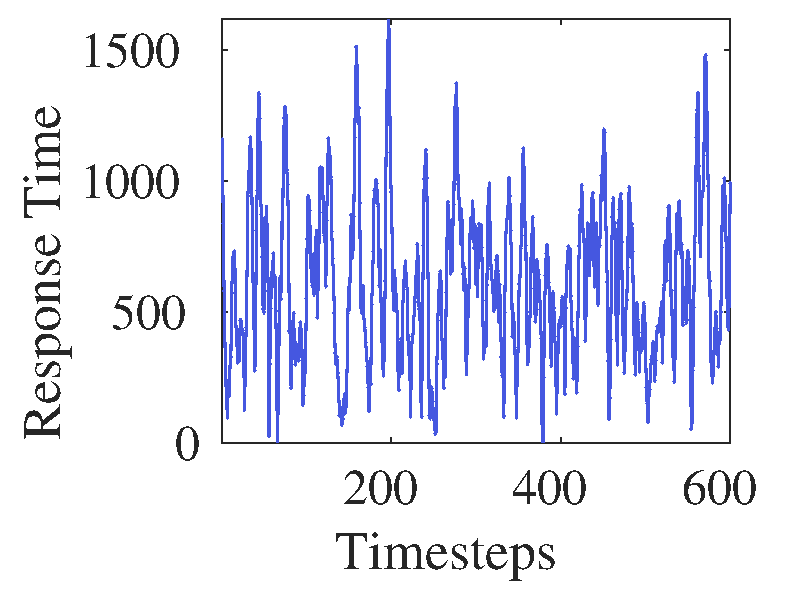
\includegraphics[scale=0.31]{Figures/Data/Uti}
  %     \label{1d}}
	\caption{Trends in datasets}
  \label{fig:trend} 
  \vspace{-3mm}
\end{figure*}

\begin{figure*}[!ht]
    \centering
  \subfloat[Fire]{%
       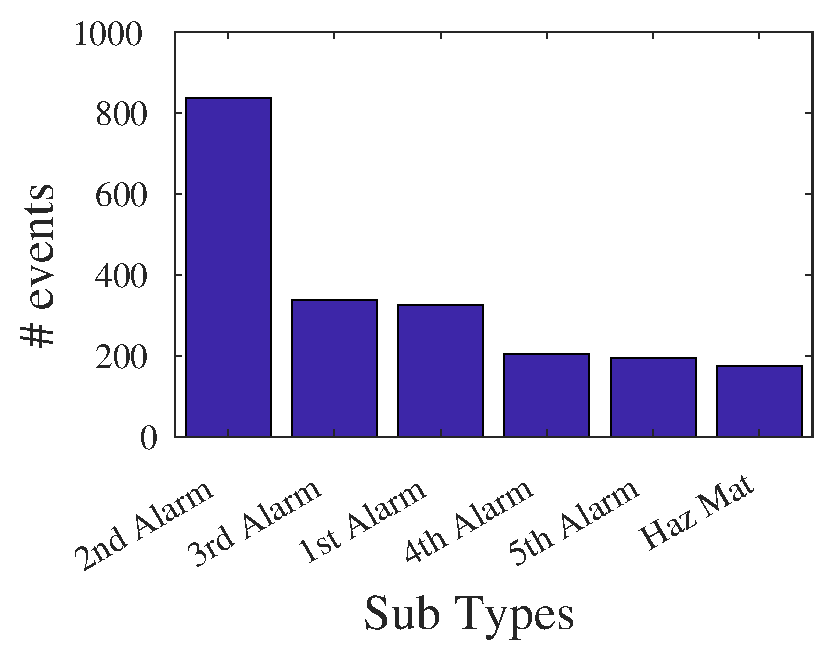
\includegraphics[scale=0.35]{Figures/Data/SubType/fire}
       \label{2a}}
       %\vspace{5mm}
  \subfloat[Law]{%
       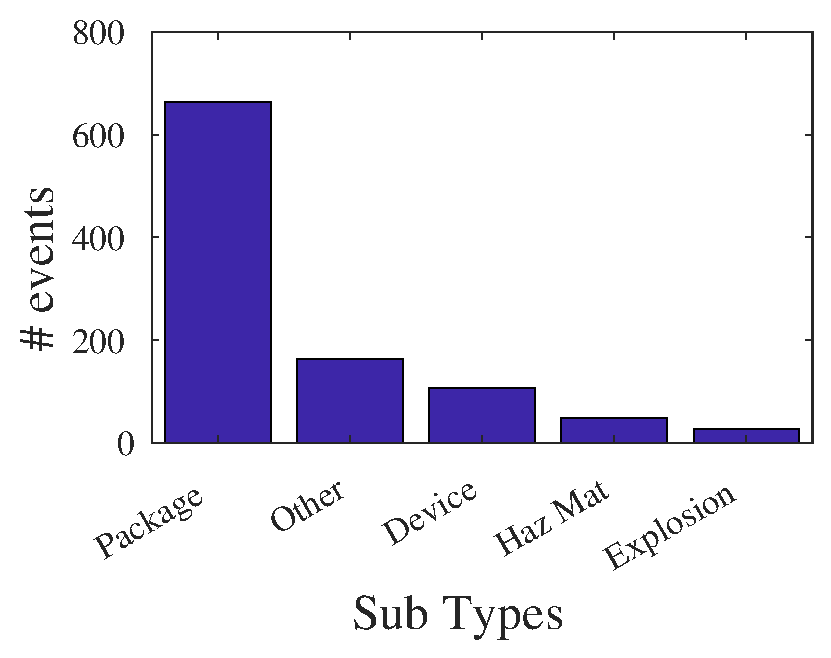
\includegraphics[scale=0.35]{Figures/Data/SubType/law}
       \label{2b}}
       %\vspace{5mm}
  \subfloat[Structural]{%
       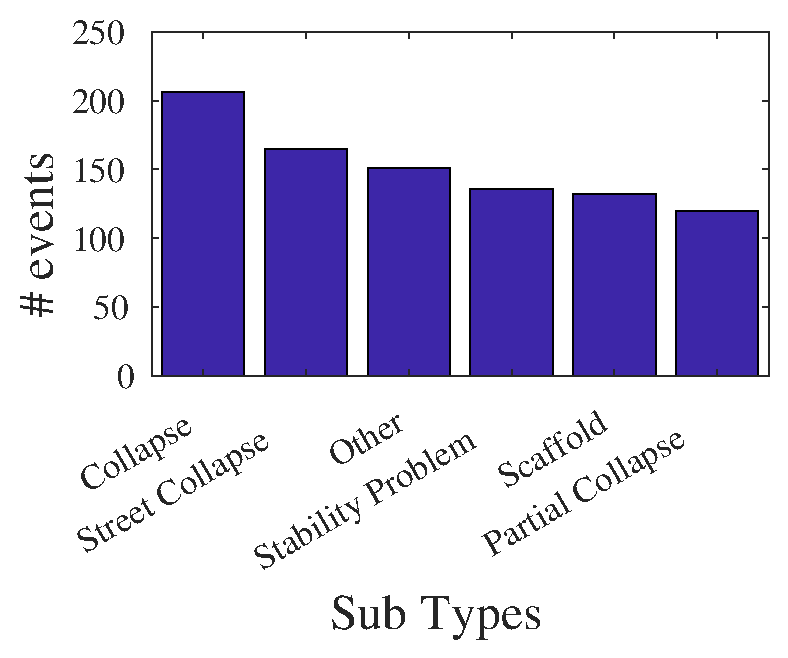
\includegraphics[scale=0.35]{Figures/Data/SubType/structural}
       \label{2c}}
  %\subfloat[Utility]{%
  %     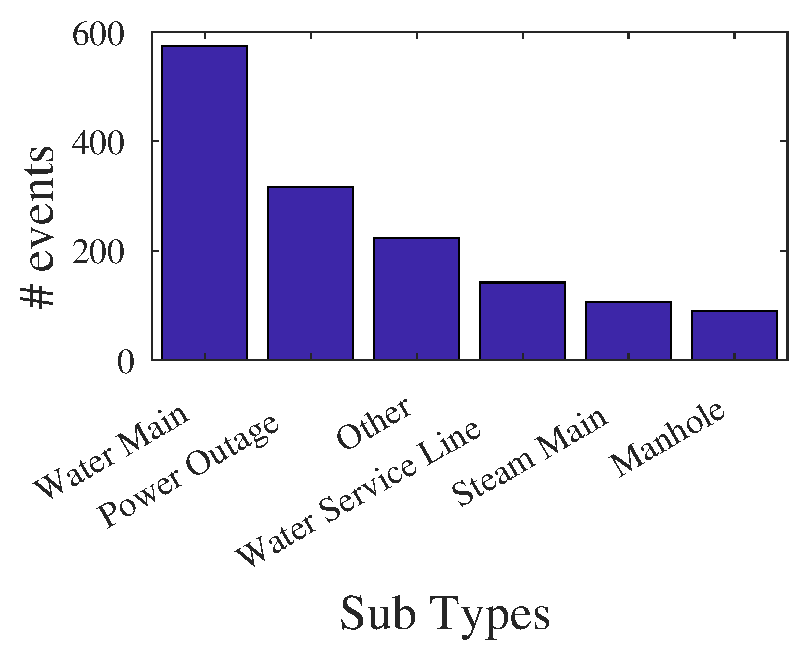
\includegraphics[scale=0.31]{Figures/Data/SubType/utility}
  %     \label{2d}}
	\caption{Incident Types}
  \label{fig:subtype} 
  \vspace{-3mm}
\end{figure*}
